%%%%%%%%%%%%%%%%%%%%%%%%%%%%%%%%%%%%%%%%%
% Beamer Presentation
% LaTeX Template
% Version 1.0 (10/11/12)
%
% This template has been downloaded from:
% http://www.LaTeXTemplates.com
%
% License:
% CC BY-NC-SA 3.0 (http://creativecommons.org/licenses/by-nc-sa/3.0/)
%
%%%%%%%%%%%%%%%%%%%%%%%%%%%%%%%%%%%%%%%%%

\documentclass{beamer}

\mode<presentation> {

\usetheme{Madrid}

\setbeamertemplate{navigation symbols}{} % Remove the navigation symbols from the bottom of all slides
}

\usepackage{chronology}
\usepackage{graphicx} % Allows including images
\definecolor{links}{HTML}{2A1B81}
\hypersetup{colorlinks,linkcolor=,urlcolor=links}

\graphicspath{ {./images/} }

%----------------------------------------------------------------------------------------
% TITLE PAGE
%----------------------------------------------------------------------------------------

\title[Rust]{Rust} % The short title appears at the bottom of every slide, the full title is only on the title page
\author{Carlos A Molina}
\date{May 4, 2022}

\begin{document}

\begin{frame}
\titlepage % Print the title page as the first slide
\end{frame}

\begin{frame}
\frametitle{Table of contents}
\tableofcontents % Throughout your presentation, if you choose to use \section{} and \subsection{} commands, these will automatically be printed on this slide as an overview of your presentation
\end{frame}

%----------------------------------------------------------------------------------------
% PRESENTATION SLIDES
%----------------------------------------------------------------------------------------

%------------------------------------------------
\section{Introduction} % Sections can be created in order to organize your presentation into discrete blocks, all sections and subsections are automatically printed in the table of contents as an overview of the talk
%------------------------------------------------

\begin{frame}

\frametitle{Logo and mascot}

\begin{columns}[c] % The "c" option specifies centered vertical alignment while the "t" option is used for top vertical alignment

\column{.45\textwidth}

  \begin{figure}
    \centering
    \href{https://foundation.rust-lang.org/img/rust-logo-blk.svg}
      {
\includegraphics[width=0.5\textwidth]{rust-logo-blk.png}}
    \caption{Rust logo}
  \end{figure}

\column{.5\textwidth}
  \begin{figure}
    \centering
    \href{https://rustacean.net/assets/rustacean-orig-noshadow.svg}
      {
\includegraphics[width=0.5\textwidth]{rustacean-orig-noshadow.png}}
    \caption{Ferris the crab. Unofficial mascot}
  \end{figure}

\end{columns}

\end{frame}

\begin{frame}
\frametitle{History}

\begin{itemize}
\item 2006. Started by Graydon Hoare as a personal project.
\item 2009. Mozilla began sponsoring the project.
\item 2012. First numbered pre-alpha release.
\item 2015. First stable release, Rust 1.0.
\item 2020. Mozilla COVID-19 layoffs raised concerns about its future.
\item 2021. Rust Foundation by AWS, Huawei, Google, Microsoft and Mozilla.
\end{itemize}

\end{frame}

\begin{frame}
\frametitle{History}

\begin{chronology}[5]{2004}{2021}{\textwidth}
    \event{2006}{Personal project}
    \event{2009}{Mozilla sponsoring}
    \event{2010}{First appearing}
    \event{2012}{Pre-alpha release}
    \event{2015}{Rust 1.0}
    \event{2020}{COVID-19 layoffs}
    \event{2021}{Rust Foundation}
\end{chronology}

\begin{columns}[c] % The "c" option specifies centered vertical alignment while the "t" option is used for top vertical alignment

\column{.3\textwidth}

  \begin{figure}
    \centering
    \href{https://github.com/graydon}
      {
\includegraphics[width=0.35\textwidth]{graydon-github.png}}
    \caption{Graydon Hoare}
  \end{figure}

\column{.7\textwidth}
  \begin{figure}
    \centering
    \href{https://foundation.rust-lang.org/members/}
      {
\includegraphics[width=0.5\textwidth]{rust-foundation-founding-members.png}}
    \caption{Rust Foundation founding members}
  \end{figure}

\end{columns}

\end{frame}

\section{Features}

\begin{frame}
\frametitle{Features}

\begin{itemize}
\item Compiled
\item Memory management
\item Cargo: cargo build, cargo fmt...
\end{itemize}

\end{frame}

\begin{frame}
\frametitle{Adoption}
\begin{itemize}
\item 2021. Google da soporte a Rust en `Android Open Source Project` como alternativa a C/C++.
\item https://www.nature.com/articles/d41586-020-03382-2
\item Dropbox created a new sync engine called Nucleus: file modifications can raise concurrency bugs
\end{itemize}

\end{frame}

\section{Demo}

\begin{frame}
\frametitle{Demo}

\begin{columns}[c] % The "c" option specifies centered vertical alignment while the "t" option is used for top vertical alignment

\column{.5\textwidth}
  \begin{figure}
    \centering
    \frame{
      \href{https://doc.rust-lang.org/stable/book/ch20-00-final-project-a-web-server.html}
	  {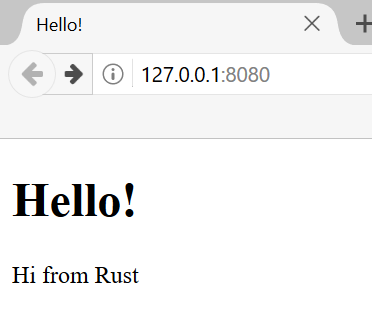
\includegraphics[width=0.7\textwidth]{trpl20-01.png}}
    }
  \caption{Web Server}
  \end{figure}

\column{.45\textwidth}
\begin{itemize}
\item Single-Threated
\item Multithreated
\end{itemize}

\end{columns}

\end{frame}

\section{References}

\begin{frame}
\frametitle{References}
\begin{itemize}
\item History and adoption\\
\href{https://en.wikipedia.org/wiki/Rust_(programming_language)}{https://en.wikipedia.org}
\item Why scientists are turning to Rust\\
\href{https://www.nature.com/articles/d41586-020-03382-2}{https://www.nature.com}
\item Dropbox adoption\\
\href{https://dropbox.tech/infrastructure/rewriting-the-heart-of-our-sync-engine}{https://dropbox.tech}
\end{itemize}
\end{frame}

\begin{frame}
\frametitle{References. Images}
\begin{itemize}
\item Rust logo\\
\href{https://foundation.rust-lang.org/policies/logo-policy-and-media-guide/\#the-rust-trademarks}{https://foundation.rust-lang.org}
\item Ferris the crab, unofficial mascot\\
\href{https://rustacean.net}{https://rustacean.net}
\item Graydon Hoare\\
\href{https://github.com/graydon}{https://github.com/graydon}
\item Rust Foundation founding members\\
\href{https://foundation.rust-lang.org/members/}{https://foundation.rust-lang.org}
\item Multithreaded Web Server\\
\href{https://doc.rust-lang.org/stable/book/ch20-00-final-project-a-web-server.html}{https://doc.rust-lang.org}
\end{itemize}
\end{frame}


\begin{frame}
\Huge{\centerline{Thank you!}}
\end{frame}

\end{document} 
